%=====================================================
\begin{frame}{2.1.3. Признание ценности сотрудничества и доверия (группы по квалификационной категории) }

\tiny

На диаграммах представлен результат по вопросам Б13, Б14 с разбивкой по квалификационной категории:
\bigskip

\centering 

\begin{tabular}{|l|c|c|c|c|c|} \hline
  & Не проходил &  Аттестован & 2-я &  1-я  & Высшая \\ 
 &  аттестацию   &  на соотв. & категория &  категория  & категория \\ \hline
Ответили  & & & & & \\
утвердительно  & \valBACyesNumA  &  \valBACyesNumB  & \valBACyesNumC  & \valBACyesNumD  & \valBACyesNumE \\ 
(Да, cкорее да...) & & & & & \\ \hline
Ответили   & & & & & \\
отрицательно & \valBACnoNumA   & \valBACnoNumB  & \valBACnoNumC  & 
\valBACnoNumD & \valBACnoNumE \\ 
(Нет, cкорее нет...) & & & & & \\ \hline
\end{tabular}

\bigskip

\begin{tabular}{ccccc}
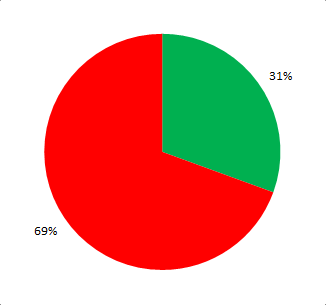
\includegraphics[width=2cm, height=2cm]{diag.png} & 
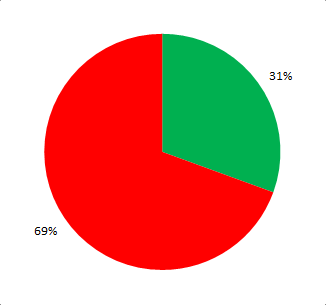
\includegraphics[width=2cm, height=2cm]{diag.png} & 
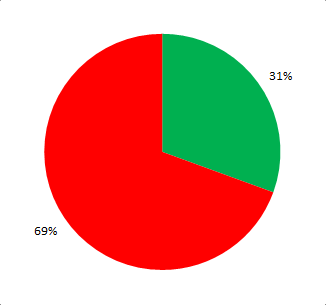
\includegraphics[width=2cm, height=2cm]{diag.png} & 
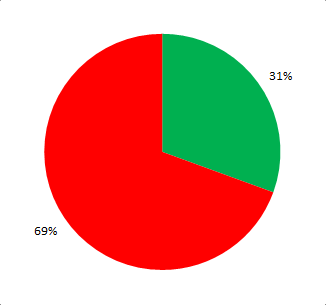
\includegraphics[width=2cm, height=2cm]{diag.png} & 
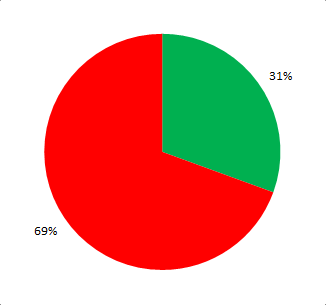
\includegraphics[width=2cm, height=2cm]{diag.png} \\
 Не проходили &  Аттестованы & 2-я &  1-я  & Высшая \\ 
  аттестацию   &  на соотв. & категория &  категория  & категория \\ 
\end{tabular}

\end{frame}


